\documentclass[tikz,border=8pt]{standalone}
\begin{document}
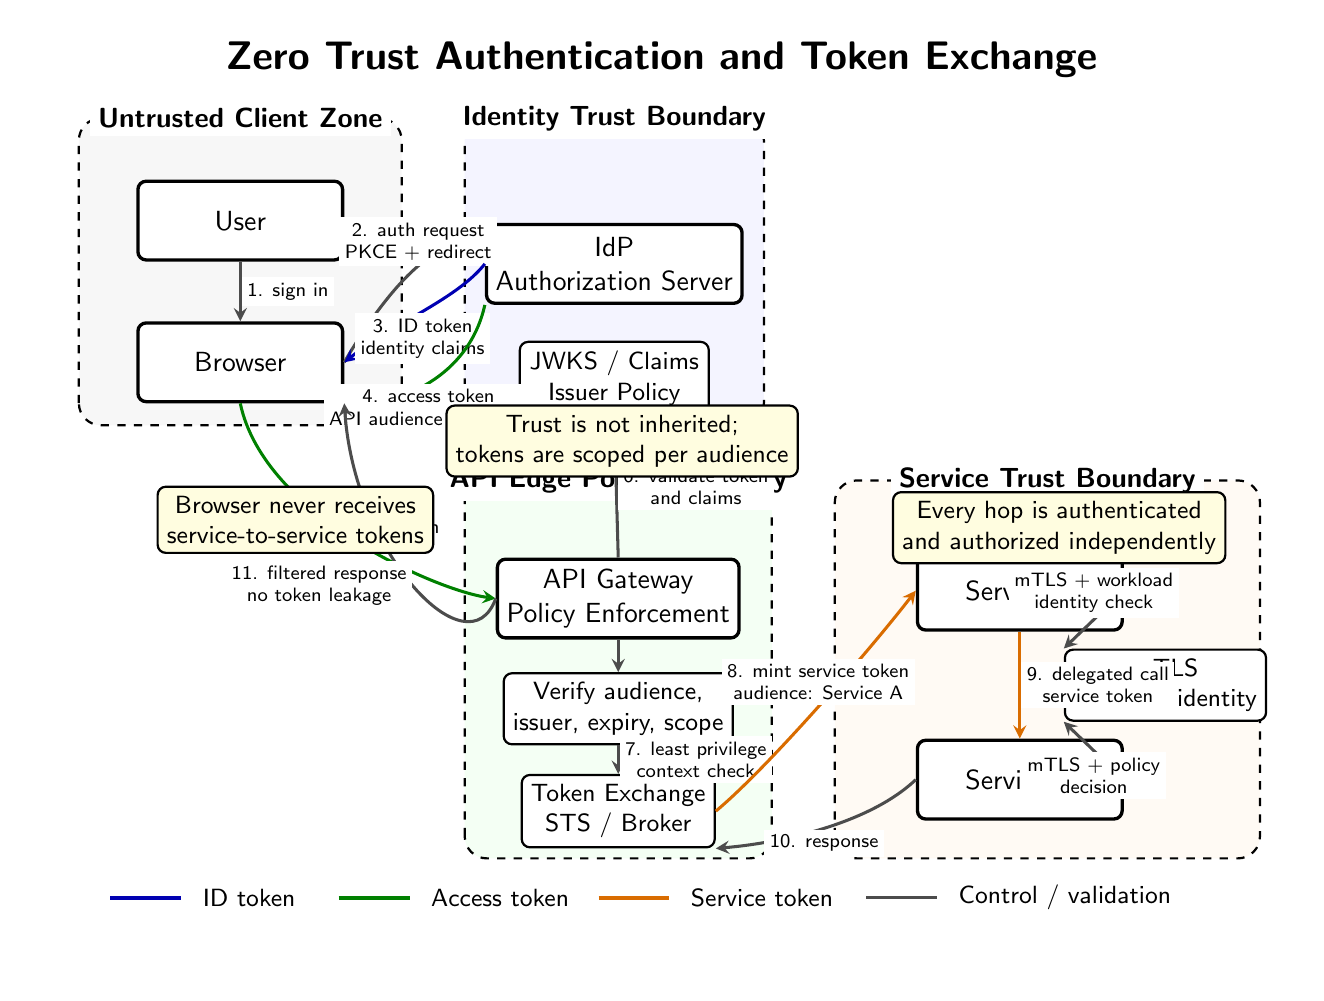
\begin{tikzpicture}[
  x=1cm,y=1cm,
  font=\sffamily,
  actor/.style={draw, rounded corners=3pt, fill=white, very thick, minimum width=2.6cm, minimum height=1.0cm, align=center},
  smallbox/.style={draw, rounded corners=3pt, fill=white, thick, minimum width=2.4cm, minimum height=.72cm, align=center, font=\sffamily\small},
  boundary/.style={draw, rounded corners=8pt, thick, dashed, fill=#1, fill opacity=.12},
  labelbox/.style={fill=white, inner sep=3pt, font=\sffamily\bfseries},
  flow/.style={->, >=stealth, line width=1.1pt},
  idtok/.style={flow, draw=blue!70!black},
  acctok/.style={flow, draw=green!50!black},
  svctok/.style={flow, draw=orange!85!black},
  control/.style={flow, draw=black!70},
  note/.style={font=\sffamily\scriptsize, align=center, fill=white, inner sep=2pt}
]

% Canvas: about 4:3 composition, suitable for 1200x900 rendering.
\path[use as bounding box] (-.4,-.4) rectangle (15.7,11.6);

% Title
\node[font=\sffamily\bfseries\Large] at (7.65,11.2)
  {Zero Trust Authentication and Token Exchange};

% Trust boundaries
\draw[boundary=gray!50] (.25,6.55) rectangle (4.35,10.45);
\node[labelbox] at (2.3,10.45) {Untrusted Client Zone};

\draw[boundary=blue!35] (5.15,6.55) rectangle (8.95,10.45);
\node[labelbox] at (7.05,10.45) {Identity Trust Boundary};

\draw[boundary=green!35] (5.15,1.05) rectangle (9.05,5.85);
\node[labelbox] at (7.1,5.85) {API Edge Policy Boundary};

\draw[boundary=orange!35] (9.85,1.05) rectangle (15.25,5.85);
\node[labelbox] at (12.55,5.85) {Service Trust Boundary};

% Components
\node[actor] (user) at (2.3,9.15) {User};
\node[actor] (browser) at (2.3,7.35) {Browser};

\node[actor] (idp) at (7.05,8.6) {IdP\\Authorization Server};
\node[smallbox] (jwks) at (7.05,7.15) {JWKS / Claims\\Issuer Policy};

\node[actor] (gw) at (7.1,4.35) {API Gateway\\Policy Enforcement};
\node[smallbox] (verify) at (7.1,2.95) {Verify audience,\\issuer, expiry, scope};
\node[smallbox] (exchange) at (7.1,1.65) {Token Exchange\\STS / Broker};

\node[actor] (svcA) at (12.2,4.45) {Service A};
\node[actor] (svcB) at (12.2,2.05) {Service B};
\node[smallbox] (mesh) at (14.05,3.25) {mTLS\\workload identity};

% Legend
\draw[blue!70!black, line width=1.3pt] (.65,.55) -- (1.55,.55);
\node[anchor=west, font=\sffamily\small] at (1.7,.55) {ID token};
\draw[green!50!black, line width=1.3pt] (3.55,.55) -- (4.45,.55);
\node[anchor=west, font=\sffamily\small] at (4.6,.55) {Access token};
\draw[orange!85!black, line width=1.3pt] (6.85,.55) -- (7.75,.55);
\node[anchor=west, font=\sffamily\small] at (7.9,.55) {Service token};
\draw[black!70, line width=1.1pt] (10.25,.55) -- (11.15,.55);
\node[anchor=west, font=\sffamily\small] at (11.3,.55) {Control / validation};

% User interaction
\draw[control] (user) -- node[note, right] {1. sign in} (browser);

% OIDC auth flow
\draw[control] (browser.east) .. controls (4.2,8.35) and (4.95,9.15) ..
  node[note, above] {2. auth request\\PKCE + redirect} (idp.west);

\draw[idtok] (idp.west) .. controls (5.05,8.15) and (4.25,7.85) ..
  node[note, below] {3. ID token\\identity claims} (browser.east);

\draw[acctok] (idp.south west) .. controls (5.2,7.15) and (4.3,6.8) ..
  node[note, below] {4. access token\\API audience + scopes} (browser.south east);

% Gateway validation
\draw[acctok] (browser.south) .. controls (2.6,5.4) and (4.8,4.45) ..
  node[note, above] {5. API request\\Bearer access token} (gw.west);

\draw[control] (gw.north) -- node[note, right] {6. validate token\\and claims} (jwks.south);
\draw[control] (gw.south) -- (verify.north);
\draw[control] (verify.south) -- node[note, right] {7. least privilege\\context check} (exchange.north);

% Token exchange and service calls
\draw[svctok] (exchange.east) .. controls (9.0,2.2) and (10.3,3.7) ..
  node[note, above] {8. mint service token\\audience: Service A} (svcA.west);

\draw[svctok] (svcA.south) -- node[note, right] {9. delegated call\\service token} (svcB.north);

\draw[control] (svcA.east) -- node[note, above] {mTLS + workload\\identity check} (mesh.north west);
\draw[control] (svcB.east) -- node[note, below] {mTLS + policy\\decision} (mesh.south west);

% Response path
\draw[control] (svcB.west) .. controls (10.3,1.5) and (9.2,1.25) ..
  node[note, below] {10. response} (exchange.south east);

\draw[control] (gw.west) .. controls (5.2,3.4) and (3.75,4.9) ..
  node[note, left] {11. filtered response\\no token leakage} (browser.south east);

% Security callouts
\node[smallbox, fill=yellow!12, minimum width=3.5cm] at (12.7,5.25)
  {Every hop is authenticated\\and authorized independently};

\node[smallbox, fill=yellow!12, minimum width=3.4cm] at (3.0,5.35)
  {Browser never receives\\service-to-service tokens};

\node[smallbox, fill=yellow!12, minimum width=3.5cm] at (7.15,6.35)
  {Trust is not inherited;\\tokens are scoped per audience};

\end{tikzpicture}
\end{document}
